\documentclass[letterpaper,twocolumn,10pt]{article}

% Standalone review doc, NOT the paper itself: dumps every figs/*.tex
% fragment for visual inspection, one section per fragment, in a fixed
% order. Regenerated by NEW_PAPER_DATA.py's "figs" top-level choice.

\usepackage{booktabs}
\usepackage{amsmath}
\usepackage{tikz}
\usepackage{pgfplots}
\pgfplotsset{compat=1.18}
\usepackage{hyperref}

\def\ttt#1{\texttt{#1}}

\title{BORA paper-data: figure/table review}
\author{}
\date{\today}

\begin{document}
\maketitle

\section*{datasets}
% Dna drop provenance (source of the 65 dropped: data/src_sig/chr17_variants/docs/reef_regex.log):
%   27565 pathogenic/likely-pathogenic chr17 variants processed; 65 skipped (63 ambiguous base (N) in allele; 2 no ALT (identity record)); 27500 kept = Rules cell.
% Auto-generated by data/scripts/eval/datasets.py -- do not edit by hand.
% Dataset characterization table for §6.2 (tab:datasets).
% All three rows are auto-extracted from the project corpus: Mal from ClamAV
% main.dat + binexec_merged128k, Dna from chr17_variants, Dlp from the
% RE2-screened Enron listing (any_server/corpus.tgz) + MS-DLP
% regex_zombie_international/ for the rule count and the jet1tb Zombie log
% for the pattern bytes. Locked layout:
% label stub outside both groups; two \multicolumn spans (Document corpus |
% Regex set); descriptive only -- NO tier (CP/SDE/DFA) columns, NO PCRE column,
% NO rule-shape column (shape facts moved to the §6.2 prose).
%
% CentOS version: the table reports the neutral "CentOS 7" only. Binary
% provenance in the corpus points to the CentOS 7.9 update stream -- bundled
% shared objects carry the RPM dist tag el7_9 (e.g. ...base.el7_9.1.so) and
% the kernel is the 3.10.0-1160 series (shipped with 7.9). \cite{Zkreg} cited
% CentOS 7.1, and no /etc/centos-release or ISO is on disk to settle the
% minor version, so we leave it at "CentOS 7" rather than commit to 7.1 or 7.9.
\begin{table*}[t]
  \centering
  \footnotesize
  \caption{Evaluation datasets: \textsc{Mal} (malware scanning), \textsc{Dna}
  (genomic variants), and \textsc{Dlp} (e-mail DLP).}
  \label{tab:datasets}
  \begin{tabular}{@{}l l r r l l r r@{}}
    \toprule
     & \multicolumn{4}{c}{Document corpus}
       & \multicolumn{3}{c}{Regex set} \\
    \cmidrule(lr){2-5} \cmidrule(lr){6-8}
     & Corpus & Docs & Size & Per-doc (min/med/max)
       & Ruleset (ver.) & Rules & Size \\
    \midrule
    \textsc{Mal} & CentOS 7 & 1{,}209 & 765\,MB & 66\,KB / 130\,KB / 33\,MB
        & ClamAV 0.103.11 & 38{,}875 & 11.6\,MB \\
    \textsc{Dna} & \begin{tabular}[t]{@{}l@{}}chr17\\(GRCh38)\end{tabular} & 1 & 83\,MB & ---~(single)
        & NCBI ClinVar (chr17) & 27{,}500 & 1.4\,MB \\
    \textsc{Dlp} & \begin{tabular}[t]{@{}l@{}}Enron\\Email\end{tabular} & 509{,}610 & 1.38\,GB & 398\,B / 1.5\,KB / 1.7\,MB
        & MS-DLP (SIT) & 136 & 213\,KB \\
    \bottomrule
  \end{tabular}
\end{table*}

\clearpage

\section*{effectiveness\_tab}
\begin{table}[t]
\centering
\footnotesize
\begin{tabular}{l r r r r}
\hline
Dataset & Pairs & $\mathtt{CP}$ & $\mathtt{SDE}$ & $\mathtt{DFA}$ \\
\hline
\textsc{Mal} & $4.70\times10^{7}$ & $99.8803\%$ & $0.1144\%$ & $0.0053\%$ \\
\textsc{Dna} & $2.75\times10^{4}$ & $99.9382\%$ & $0.0618\%$ & $0.0000\%$ \\
\textsc{Dlp} & $4.98\times10^{9}$ & $99.9980\%$ & $0.0020\%$ & $0.0000\%$ \\
\hline

\end{tabular}
\caption{Tier-discharge fractions per dataset.}
\label{tab:eff-pair}
\end{table}
\clearpage

\section*{effectiveness\_size}
\begin{table}[t]
\centering
\footnotesize
\begin{tabular}{l r r r r}
\hline
Size (B) & Files & $\mathtt{CP}$ & $\mathtt{SDE}$ & $\mathtt{DFA}$ \\
\hline
$2^{16}$--$2^{19}$ & 954 & $99.9140\%$ & $0.0808\%$ & $0.0052\%$ \\
$2^{19}$--$2^{21}$ & 220 & $99.7566\%$ & $0.2380\%$ & $0.0054\%$ \\
$2^{21}$--$2^{23}$ & 21 & $99.8119\%$ & $0.1809\%$ & $0.0072\%$ \\
$2^{23}$--$2^{25}$ & 14 & $99.6333\%$ & $0.3577\%$ & $0.0090\%$ \\
\hline

\end{tabular}
\caption{Tier-discharge fractions by file size (Mal).}
\label{tab:eff-size}
\end{table}
\clearpage

\section*{effectiveness\_size\_dlp}
\begin{table}[t]
\centering
\footnotesize
\begin{tabular}{l r r r r}
\hline
Size (B) & Files & $\mathtt{CP}$ & $\mathtt{SDE}$ & $\mathtt{DFA}$ \\
\hline
$2^{7}$--$2^{11}$ & 326235 & $99.9992\%$ & $0.0008\%$ & $0.0000\%$ \\
$2^{11}$--$2^{14}$ & 172337 & $99.9965\%$ & $0.0035\%$ & $0.0000\%$ \\
$2^{14}$--$2^{17}$ & 6130 & $99.9793\%$ & $0.0207\%$ & $0.0000\%$ \\
$2^{17}$--$2^{20}$ & 152 & $99.9384\%$ & $0.0616\%$ & $0.0000\%$ \\
\hline

\end{tabular}
\caption{Same, over Dlp.}
\label{tab:eff-size-dlp}
\end{table}
\clearpage

\section*{lookup}
\begin{table*}[t]
\centering
\small
\setlength{\tabcolsep}{4pt}
\begin{tabular}{@{}ll rr rr rr@{}}
\toprule
 & & \multicolumn{2}{c}{\textsc{Mal}} & \multicolumn{2}{c}{\textsc{Dna}} & \multicolumn{2}{c}{\textsc{Dlp}} \\
\cmidrule(lr){3-4}\cmidrule(lr){5-6}\cmidrule(lr){7-8}
Component & Purpose & M & \% & M & \% & M & \% \\
\midrule
range table$^\dagger$ & range proof e.g. for pattern distance & 67.1 & 85.9 & 134.2 & 98.4 & 33.6 & 99.6 \\
AC-DFA / CP & transition rules & 3.2 & 4.2 & 1.1 & 0.8 & 0.1 & 0.2 \\
SDE & subsig step pattern distance constraints & 7.7 & 9.9 & 1.1 & 0.8 & 0.1 & 0.2 \\
DFA (4/0/0) & transition rules & 0.1 & 0.1 & 0.0 & 0.0 & 0.0 & 0.0 \\
sig-DB & DNF combinations / tri-logic truth table & 0.0 & 0.0 & 0.0 & 0.0 & 0.0 & 0.0 \\
\midrule
TOTAL populated & & 78.2 & 29.1 & 136.4 & 50.8 & 33.7 & 12.6 \\
\#signatures & & \multicolumn{2}{c}{1,944} & \multicolumn{2}{c}{1,375} & \multicolumn{2}{c}{494} \\
\bottomrule
\end{tabular}
\caption{Lookup-table composition across datasets. Column \emph{M} is millions of entries. Each \% is of that dataset's populated entries; TOTAL \% is of the $2^{28}$ capacity. $^\dagger$range table $=2^{\text{range2\_bit}}$ (26 / 27 / 25 for \textsc{Mal}/\textsc{Dna}/\textsc{Dlp}), sized by the maximum document offset. The $(\cdot/\cdot/\cdot)$ after \emph{DFA} is the number of DFAs folded in for rules that frequently fail SDE, per dataset.
BORA re-writes \ttt{(kw1|...kwn).\{0,N\}pat} in \textsc{Dlp} to disjunction of $n$ rules for improved SDE accuracy, thus expanding from $136$ to $9861$.}
\label{tbl:lkup}
\end{table*}

\clearpage

\section*{component\_cost}
% GENERATED by data/scripts/eval/gen_component_cost.py -- do not edit.
% Per-circuit cost profile for Q2 (component R1CS per folding step).
% Each c_i cell is `raw (adjusted)': raw = component R1CS / input byte;
% adjusted = raw after the MEASURED c4 log-up query cost (PERF 1012)
% is moved out of the framework and split across tiers by data-column
% proportion, so c1/c2/c3 become all-in and c4 keeps only Poseidon/IO.
% A `*' row lacks the per-component data-column log, so only raw is
% shown (the split is not yet available -- not accurate).
\begin{table*}[t]
\centering
\small
\setlength{\tabcolsep}{6pt}
\begin{tabular}{@{}ll r r rrrr r@{}}
\toprule
        &      & input & total  & \multicolumn{4}{c}{R1CS / input byte: raw (adjusted)}
        & corpus \\
\cmidrule(lr){5-8}
Dataset & Circ & (B)   & R1CS   & $c_1$ (CP) & $c_2$ (SDE) & $c_3$ (DFA)
        & $c_4$ (frwk) & share \\
\midrule
\textsc{Mal} & *** & *** & *** & *** & *** & *** & *** & *** \\
\midrule
\textsc{Dna} & *** & *** & *** & *** & *** & *** & *** & *** \\
\midrule
\textsc{Dlp} & *** & *** & *** & *** & *** & *** & *** & *** \\
\bottomrule
\end{tabular}
\caption{Per-circuit cost profile. Each dataset is discharged by a small set of circuits. \emph{input} is the bytes processed per folding step. Each $c_i \in (c_1,c_2,c_3,c_4)$ is the per-input-byte R1CS constraints of the four components of a circuit.Each $c_i$ is shown as \emph{raw\,(adjusted)}: the \emph{adjusted} value moves the \emph{measured} log-up query cost in $c_4$ and charges it to each tier in  proportion to its data-column size, so $c_1/c_2/c_3$ reflect the  all-in per-byte cost and $c_4$ retains only folding overhead  and the processing of Logup share of lookup table. }\label{tbl:component-cost}
\end{table*}

\clearpage

\section*{overall\_perf}
% GENERATED by data/scripts/eval/gen_overall_perf.py -- do not edit.
% Per-dataset end-to-end prover breakdown for Q3 (overall perf).
% Stage 1 (folding) = circuit-selection + commit-fixed-witness +
% folding, summed CPU-time over jobs; Total is their sum. Stage 2
% (Compression) is the per-job decider/SNARK tail (Groth16 keygen
% excluded as one-time setup). The footer row reports one batch
% proof's size and verify cost (constant in corpus/rule-set; a run
% emits one such proof per job), extracted from the
% BatchProof/IndividualProof log sections.
\begin{table*}[t]
\centering
\small
\setlength{\tabcolsep}{6pt}
\begin{tabular}{@{}l r r r rrrr r@{}}
\toprule
        &        &      &       & \multicolumn{3}{c}{Stage 1: Main Folding}
        &       & \multicolumn{1}{c}{Stage 2} \\
\cmidrule(lr){5-7}\cmidrule(lr){9-9}
Dataset & Corpus & Jobs & Steps & Sel. & Commit wit. & Fold & Total\,/\,Wall (jobs)
        & Compression \\
\midrule
\textsc{Mal} & $793.4$\,MB & $8$ & 6{,}552 & $12.74$\,hr & $14.61$\,hr & $89.64$\,hr & $116.99$\,hr\,/\,$14.62$\,hr ($8$) & $2.84$\,hr \\
\textsc{Dna} & $39.7$\,MB & $1$ & 328 & $18.0$\,min & $25.9$\,min & $2.43$\,hr & $3.16$\,hr ($1$) & $1.28$\,hr \\
\textsc{Dlp} & $1.7$\,GB & $8$ & 926{,}900 & $38.68$\,hr & $43.24$\,hr & $426.02$\,hr & $507.94$\,hr\,/\,$63.49$\,hr ($8$) & $1.76$\,hr \\
\midrule
\multicolumn{9}{@{}l}{\footnotesize Per batch proof (one per job, constant): size $1{,}152$\,B, verification $32$\,ms.} \\
\bottomrule
\end{tabular}
\caption{End-to-end prover performance. \emph{Corpus} is the bytes actually folded: \textsc{Dna} packs each base of its chr17 sequence into a nibble (half a byte), halving it to the $39.7$\,MB shown, while the $793.4$\,MB \textsc{Mal} results from padding each chunk to $128$\,KB. \emph{Stage 1} (main folding) is the corpus-scaling cost: circuit selection $+$ commit fixed witness $+$ folding. \emph{Total\,/\,Wall (jobs)} reports the summed CPU-time over the parallel jobs and the wall-clock time; for balanced jobs the wall-clock is ${\approx}\,$Total$/$Jobs. \emph{Stage 2: Compression} computes the main-circuit SNARK proof, the QA-NIZK proof, the cycle-pairing fold, and the resulting batch proof. It is a fixed per-job cost, and all timings exclude the one-time key setup. The bottom row shows the size and verification cost of one batch proof (mainly the two Groth16 SNARK proofs); this per-job batch proof is constant size and independent of corpus and rule-set size. A run emits one batch proof per job, as jobs split a corpus to save wall time.}
\label{tbl:overall-perf}
\end{table*}

\clearpage

\section*{scale}
% GENERATED by data/scripts/eval/gen_scale_all.py -- do not edit.
% Q4 scalability in regex-set size (input fixed), per folding step.
% Two-column figure*: columns = datasets (ClamAV | MS-DLP), rows =
% metrics (top: absolute R1CS with single-rule floor; bottom: net R1CS
% per rule-byte). One curve per corpus (dense / sparse). Lookup share
% excluded (one-time, amortized). All numbers derived from logs.
\begin{figure*}[t]
\centering
\begin{minipage}[t]{\columnwidth}
\centering
{\small \textsc{ClamAV}}\par
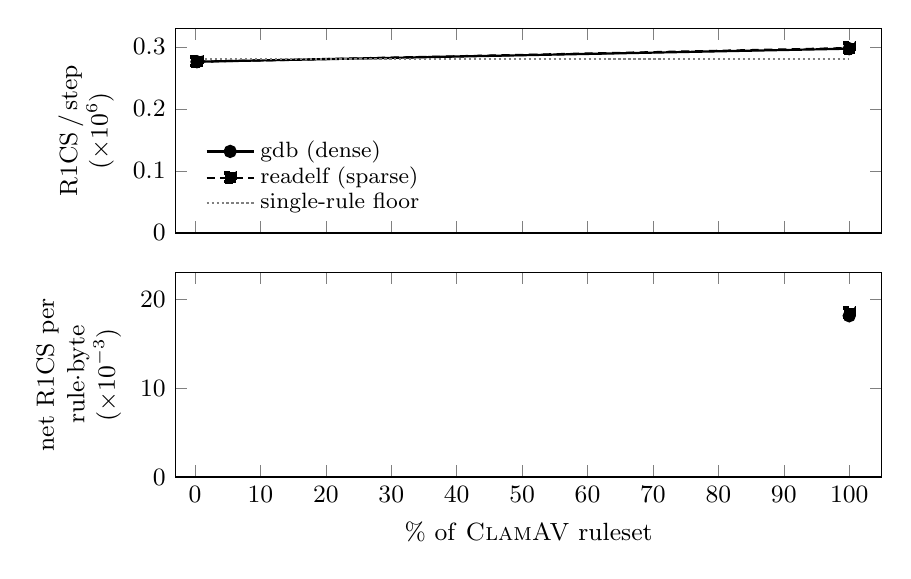
\begin{tikzpicture}[baseline=(ptop.north west)]
% --- top: absolute per-step circuit size ---
\begin{axis}[
    name=ptop, scale only axis, width=0.74\columnwidth, height=2.6cm,
    xmin=-3, xmax=105, xtick={0,10,20,30,40,50,60,70,80,90,100}, xticklabels={},
    ymin=0, ymax=0.33, ylabel={R1CS\,/\,step\\($\times10^{6}$)}, ylabel style={font=\small, align=center}, 
    tick label style={font=\small}, label style={font=\small},
    legend style={font=\footnotesize, at={(0.03,0.04)}, anchor=south west, draw=none, fill=none, row sep=-2pt}, legend cell align=left]
  \addplot[mark=*, thick] coordinates {(0.3,0.276)(100.0,0.297)};
  \addlegendentry{gdb (dense)}
  \addplot[mark=square*, thick, densely dashed] coordinates {(0.3,0.276)(100.0,0.298)};
  \addlegendentry{readelf (sparse)}
  \addplot[gray, densely dotted, thick] coordinates {(0,0.28)(100,0.28)};
  \addlegendentry{single-rule floor}
\end{axis}
% --- bottom: net R1CS per rule-byte (amortization) ---
\begin{axis}[
    name=pbot, scale only axis, width=0.74\columnwidth, height=2.6cm,
    at={(ptop.south west)}, anchor=north west, yshift=-0.5cm,
    xmin=-3, xmax=105, xtick={0,10,20,30,40,50,60,70,80,90,100},
    xlabel={\% of \textsc{ClamAV} ruleset},
    ymin=0, ymax=23.0, ylabel={net R1CS per\\rule$\cdot$byte\\($\times10^{-3}$)}, ylabel style={font=\small, align=center}, 
    tick label style={font=\small}, label style={font=\small}]
  \addplot[mark=*, thick] coordinates {(100.0,18.115)};
  \addplot[mark=square*, thick, densely dashed] coordinates {(100.0,18.423)};
\end{axis}
\end{tikzpicture}
\end{minipage}
\hfill
\begin{minipage}[t]{\columnwidth}
\centering
{\small \textsc{MS-DLP}}\par
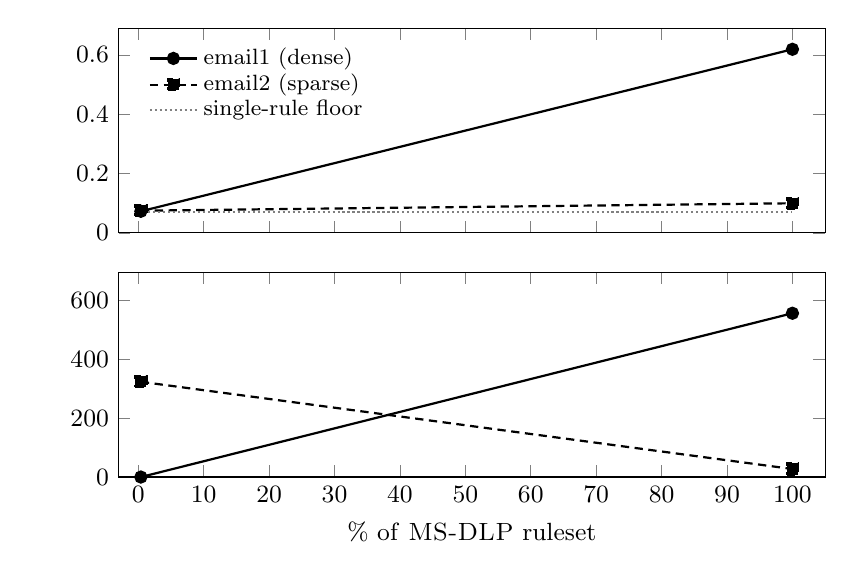
\begin{tikzpicture}[baseline=(ptop.north west)]
% --- top: absolute per-step circuit size ---
\begin{axis}[
    name=ptop, scale only axis, width=0.74\columnwidth, height=2.6cm,
    xmin=-3, xmax=105, xtick={0,10,20,30,40,50,60,70,80,90,100}, xticklabels={},
    ymin=0, ymax=0.69, yticklabel style={text width=2.6em, align=right}, 
    tick label style={font=\small}, label style={font=\small},
    legend style={font=\footnotesize, at={(0.03,0.96)}, anchor=north west, draw=none, fill=none, row sep=-2pt}, legend cell align=left]
  \addplot[mark=*, thick] coordinates {(0.4,0.073)(100.0,0.619)};
  \addlegendentry{email1 (dense)}
  \addplot[mark=square*, thick, densely dashed] coordinates {(0.4,0.075)(100.0,0.100)};
  \addlegendentry{email2 (sparse)}
  \addplot[gray, densely dotted, thick] coordinates {(0,0.07)(100,0.07)};
  \addlegendentry{single-rule floor}
\end{axis}
% --- bottom: net R1CS per rule-byte (amortization) ---
\begin{axis}[
    name=pbot, scale only axis, width=0.74\columnwidth, height=2.6cm,
    at={(ptop.south west)}, anchor=north west, yshift=-0.5cm,
    xmin=-3, xmax=105, xtick={0,10,20,30,40,50,60,70,80,90,100},
    xlabel={\% of \textsc{MS-DLP} ruleset},
    ymin=0, ymax=695.5, yticklabel style={text width=2.6em, align=right}, 
    tick label style={font=\small}, label style={font=\small}]
  \addplot[mark=*, thick] coordinates {(0.4,0.000)(100.0,556.387)};
  \addplot[mark=square*, thick, densely dashed] coordinates {(0.4,323.589)(100.0,27.241)};
\end{axis}
\end{tikzpicture}
\end{minipage}
\caption{Ruleset-size scalability (input fixed), per folding step, on \textsc{ClamAV} (left) and \textsc{MS-DLP} (right). \emph{Top:} absolute circuit size with the single-rule framework floor (dotted; $0.28$\,M R1CS for \textsc{ClamAV}, $0.07$\,M for \textsc{MS-DLP}); growing the ruleset to the full $300$ (\textsc{ClamAV}) / $494$ (\textsc{MS-DLP}) rules grows the circuit far slower than the rule count. \emph{Bottom:} net circuit cost \emph{per rule per input byte}---cumulative R1CS above the floor divided by cumulative rule count times per-step input length---falling from $18.11\times10^{-3}$ to $18.11\times10^{-3}$ (\ttt{gdb}) and $18.42\times10^{-3}$ to $18.42\times10^{-3}$ (\ttt{readelf}) R1CS per rule-byte (\textsc{ClamAV}) and $556.39\times10^{-3}$ to $556.39\times10^{-3}$ (\ttt{email1}) and $323.59\times10^{-3}$ to $27.24\times10^{-3}$ (\ttt{email2}) R1CS per rule-byte (\textsc{MS-DLP}) at the full set. For the same \textsc{MS-DLP} ruleset, \textsc{Zombie} emits $3{,}407{,}872$ R1CS in total; dividing by the $2000$-byte input and the same $494$ rules gives $\sim$$3.45$ R1CS per rule-byte, the same normalization applied to BORA.}
\label{fig:scale-regex}
\end{figure*}

\clearpage

\section*{dna\_reef\_bora}
% Auto-generated by data/scripts/eval/dna_reef_bora.py
% Sources (server-specific, under data/raw_data/<SERVER_TO_USE>/):
%   reef_sample_run.log
%   full_dna.tgz
%
% Why the consistency / evaluation proof (pi_poly -- the Hyrax opening of the
% document polynomial commitment) is NOT charged into net:
%   Reef's released code computes one such opening per (doc, regex) pair,
%   because its Fiat-Shamir evaluation point q_r is derived from each regex's
%   own proof transcript. That cost is, however, amortizable: a single
%   Fiat-Shamir challenge can be derived over the ENTIRE regex set, so the
%   document commitment need be opened only ONCE for the whole batch rather
%   than once per regex. We therefore treat it as a one-time per-document
%   cost (like the commitment load and SNARK setup) and exclude it from the
%   per-regex net, for both Reef and BORA.
\begin{table*}[!b]
  \centering
  \small
  \caption{Reef per-bucket cost vs.\ BORA on chr17~$\times$~NCBI (27{,}500
  regexes). Both systems are compared on the \emph{net} step-folding cost
  only, excluding commitment, setup, and IVC proof compression, for
  a fair comparison.
  For Reef, net $=$ witness generation $+$
  Nova prove $+$ SAFA solve (\texttt{fa\_solver}); it excludes the fixed
  floor (the 4.3\,GB commitment load, SNARK setup, consistency proof, and
  related one-time costs). For BORA, net $=$ the Phase~1 circuit selection
  and non-deterministic advice generation, and Phase~2 main-folding step
  cost, excluding the Groth16 IVC proof compression as well as setup and
  commitment. Estimate1 uses each bucket's measured per-run mean times its
  population count; Estimate2 uses the minimum measured per-run mean
  (proj\_512k) times bucket count as a counterfactual floor.}
  \label{tab:dna-reef-bora}
  \begin{tabular}{l r r r r}
    \toprule
    Bucket & Count & Per-run net cost (s) & Estimate1 (s) & Estimate2 (s) \\
    \midrule
    non\_projectable & 24,434 & $1036.18 \pm 0.00$ & $2.532 \times 10^{7}$ & $1.657 \times 10^{5}$ \\
    proj\_512k &     58 & $6.78 \pm 0.00$ & $3.932 \times 10^{2}$ & $3.932 \times 10^{2}$ \\
    proj\_2M &    132 & $13.54 \pm 0.00$ & $1.787 \times 10^{3}$ & $8.950 \times 10^{2}$ \\
    proj\_4M &  1,194 & $25.76 \pm 0.00$ & $3.076 \times 10^{4}$ & $8.095 \times 10^{3}$ \\
    proj\_8M &    869 & $51.70 \pm 0.00$ & $4.493 \times 10^{4}$ & $5.892 \times 10^{3}$ \\
    proj\_16M &    813 & $88.41 \pm 0.00$ & $7.188 \times 10^{4}$ & $5.512 \times 10^{3}$ \\
    \midrule
    \textbf{Reef TOTAL} & \textbf{27,500} & --- & \textbf{$2.547 \times 10^{7}$} (294.77\,d) & \textbf{$1.865 \times 10^{5}$} (2.16\,d) \\
    \textbf{BORA} & \textbf{27,500} & --- (single batched run) & \textbf{$1.170 \times 10^{4}$} (3.25\,hr) --- $\approx 2176\times$ faster & \textbf{$1.170 \times 10^{4}$} (3.25\,hr) --- $\approx 15.93\times$ faster \\
    \bottomrule
  \end{tabular}
\end{table*}

\clearpage

\section*{zombie\_data}
% Auto-generated by data/scripts/eval/gen_zombie_table.py
% Source: data/raw_data/run_zombie_regex_zombie_international.log
%
% Per-block totals over all 'ok' international SIT regex instances. The unit cost
% u = (total prove time) / (L_T * total regex bytes) is the price of one
% input-byte x one regex-byte; it is reused in tab:compare-zombie-bora to
% project the full Mal/Dna/Dlp corpora. Rows are whichever STR_LENGTHs are
% actually in the log (see _detect_str_lens); if UNIT_STR_LEN=2000 isn't
% among them (e.g. a dry-run sweep), it's linearly interpolated from the
% 1000B row -- see _linear_interp() -- and marked with a dagger.
\begin{table*}[t]
  \centering
  \small
  \caption{Zombie prover cost on the MS-DLP international SIT rules
  (Spartan NIZK, two-pattern proximity circuit), totalled over all
  4 regex instances (the 4 \textsc{Sit} rules of
  Table~\ref{tab:datasets}, expanded into their comb variants) at each
  scanned document length $L_T$. The total regex size (sum of pattern $+$
  keyword bytes over all instances, each sub-pattern counted once) is fixed
  at 7,443\,B. The last row
  derives the unit cost $u = t_{\text{prove}} / (L_T \cdot \sum s)$ in seconds
  per (input-byte $\times$ regex-byte). Rows marked $^\dagger$ have no real
  measurement at that length in this log (e.g.\ a dry-run sweep with a
  smaller \texttt{VEC\_SIZE}) -- all four totals are linearly
  interpolated from the 1{,}000\,B row, under a linear-growth
  assumption matching Zombie's per-byte circuit complexity; treat them
  as illustrative, not measured.}
  \label{tab:zombie-data}
  \begin{tabular}{r r r r r}
    \toprule
    $L_T$ (B) & Total constraints & Prove (s) & Verify (s) & Proof (MB) \\
    \midrule
    700 & 1,179,648 & 9.2 & 4.2 & 0.11 \\
    800 & 1,310,720 & 25.4 & 15.0 & 0.14 \\
    1,000 & 1,310,720 & 13.5 & 7.6 & 0.16 \\
    2,000$^\dagger$ & 2,621,440 & 27.1 & 15.3 & 0.31 \\
    \midrule
    \multicolumn{5}{l}{Unit $u = t/(L_T\cdot\sum s)$ at $L_T=700 / 800 / 1,000 / 2,000$: $1.77 \times 10^{-6} / 4.26 \times 10^{-6} / 1.82 \times 10^{-6} / 1.82 \times 10^{-6}$ s\,B$^{-2}$} \\
    \bottomrule
  \end{tabular}
\end{table*}

\clearpage

\section*{compare\_zombie\_bora}
% Auto-generated by data/scripts/eval/gen_zombie_table.py
% Sources (server-specific, under data/raw_data/<SERVER_TO_USE>/):
%   full_clam.tgz  (BORA full ClamAV, 8-job sum)
%   full_dna.tgz   (BORA full DNA, single job)
%   full_dlp.tgz   (BORA Dlp; currently a copy of the full_dna run)
%   dataset corpus + regex sizes via common extractors (same as tab:datasets)
%
% Est. Zombie = u * (corpus bytes) * (regex-set bytes), the full doc x regex
% cross product, with u the 2000-byte unit cost from
% tab:zombie-data (closest to BORA's folding step size). This UNDER-estimates
% Zombie at MB-scale documents (Spartan prove is super-linear in constraints),
% so it is charitable to Zombie. BORA = phase-1 main-circuit folding net
% (bora_net_cost): single-job DNA, 8-job sum for ClamAV. Dlp temporarily
% reuses the full_dna run (its real dump is regenerating on the server).
\begin{table*}[t]
  \centering
  \small
  \caption{Projected Zombie cost (unit $\bar u =
  1.82 \times 10^{-6}$ s\,B$^{-2}$, taken at $L_T=2,000$) vs.\ BORA's net main-circuit folding
  cost. $\text{Est.\ Zombie} = \bar u \cdot (\text{corpus})\cdot
  (\text{regex set})$, a full document~$\times$~regex cross product. Regex-set
  size is on-disk rule-file bytes for \textsc{Mal}/\textsc{Dna}; for
  \textsc{Dlp} it is the pattern$+$keyword bytes fed to the circuit (the
  on-disk \texttt{.regex} doubles each sub-pattern for the bidirectional
  proximity form). $\bar u$ itself is linearly interpolated (see Table~\ref{tab:zombie-data}'s $\dagger$ note): this log has no real measurement at $L_T=2,000$, e.g.\ a dry-run sweep. The \textsc{Mal} (ClamAV) BORA cost $130.70$\,hr is the total over its $8$ parallel jobs; the wall-clock time is $16.80$\,hr (the slowest job). The \textsc{Dlp} (Enron) BORA cost $0.23$\,hr is the total over its $2$ parallel jobs; the wall-clock time is $0.12$\,hr (the slowest job).}
  \label{tab:compare-zombie-bora}
  \begin{tabular}{l r r r r r}
    \toprule
    Dataset & Corpus & Regex set & Est.\ Zombie & BORA (net) & Speedup \\
    \midrule
    \textsc{Mal} (ClamAV) & 765.5\,MB & 11.6\,MB & $1.62 \times 10^{10}$ (513.6\,yr) & $4.71 \times 10^{5}$ (130.70\,hr) & $\approx 34,450\times$ \\
    \textsc{Dna} (chr17) & 83.3\,MB & 1.4\,MB & $2.14 \times 10^{8}$ (6.8\,yr) & $2.71 \times 10^{2}$ (0.08\,hr) & $\approx 790,573\times$ \\
    \textsc{Dlp} (Enron) & 1.42\,GB & 7.4\,KB & $1.92 \times 10^{7}$ (222.6\,d) & $8.26 \times 10^{2}$ (0.23\,hr) & $\approx 23,297\times$ \\
    \bottomrule
  \end{tabular}
\end{table*}

\clearpage

\section*{compare\_all}
% Auto-generated by data/scripts/eval/gen_compare_all.py -- do not edit by hand.
% Consolidated Zombie / Reef / BORA comparison across all three datasets,
% keyed by tag to tab:datasets (no size columns, to avoid overlap). Replaces
% the main-body role of tab:compare-zombie-bora.
%
% Provenance (all cells reuse the Table 1/3/4 extractors -- see module docstring):
%   Zombie (all):  u (zombie_totals @ 2000 B) * corpus * regex set.
%   Reef Dna:      parse_reef_log -- Estimate1 (as-impl) / Estimate2 (floor).
%   Reef Mal/Dlp:  cheapest measured Dna per-run cost * rule count * corpus.
%   BORA all:      bora_cost_breakdown net (8-job sum / single); wall = slowest.
%                  Dlp temporarily reuses the full_dna run (real dump pending).
\begin{table*}[t]
  \centering
  \small
  \caption{End-to-end prover cost of Zombie~\cite{Zombie23},
  Reef~\cite{Reef}, and BORA on the three datasets of
  Table~\ref{tab:datasets}; the last two columns give BORA's speedup over
  each. Zombie costs are projected from the unit cost
  $u=5.09 \times 10^{-6}$~s\,B$^{-2}$ (Table~\ref{tab:zombie-data}). For
  \textsc{Dna}, Reef's as-implemented cost is shown with its optimistic
  floor in parentheses. Values marked $^{*}$ are projected from Reef's
  cheapest measured per-run cost on \textsc{Dna}
  ($7.33$\,s, the \texttt{proj\_512k} bucket):
  the \textsc{Dna} floor as that cost per signature, and Reef
  \textsc{Mal}/\textsc{Dlp} as that cost per signature per corpus byte
  (Table~\ref{tab:dna-reef-bora}). \textsc{Mal} BORA is the total net cost summed over $8$ parallel jobs; the wall-clock time is $16.80$\,hr (the slowest job). \textsc{Dlp} BORA is the total net cost summed over $8$ parallel jobs; the wall-clock time is $119.03$\,hr (the slowest job). Cells shown as ``??'' have no
  audited measurement yet.}
  \label{tab:compare-all}
  \begin{tabular}{l r r r r r}
    \toprule
    Dataset & Zombie & Reef & BORA
      & \multicolumn{2}{c}{Speedup} \\
    \cmidrule(lr){5-6}
    & & & & vs Zombie & vs Reef \\
    \midrule
    \textsc{Mal} & 1436.9\,yr & 6.9\,Myr$^{*}$ & 130.70\,hr & $96{,}375\times$ & $464\text{M}\times^{*}$ \\
    \textsc{Dna} & 19.0\,yr & 300.9\,d (2.3\,d$^{*}$) & 3.25\,hr & $51{,}148\times$ & $2{,}222\times$ ($17\times^{*}$) \\
    \textsc{Dlp} & 48.8\,yr & 44{,}894\,yr$^{*}$ & 916.95\,hr & $467\times$ & $429{,}187\times^{*}$ \\
    \bottomrule
  \end{tabular}
\end{table*}


\end{document}
